\documentclass[aspectratio=169,
				xcolor=table]{beamer}

% Load general definitions
\usepackage[utf8]{inputenc}
%\usepackage[T1]{fontenc}
\usepackage[brazil]{babel}
\usepackage{amsmath}
\usepackage{amsfonts}
\usepackage{amssymb}
\usepackage{graphicx}
\usepackage{verbatim}
\usepackage{cancel}
\usepackage{askmaps}
\usepackage{tabularx}
\usepackage[table]{xcolor}
%\usepackage{tikz}
\usepackage{multirow}
\usepackage{mathtools}
\usepackage{color, colortbl}
\usepackage{etoolbox}
\usepackage{pbox}
\usepackage{changepage}
\usepackage{xpatch}
\usepackage{array}
\usepackage{marvosym}
\usepackage{tabu}
\usepackage{multicol}
\usepackage{listings}
\usepackage{underscore}
\usepackage{filecontents}
\usepackage[]{algorithm2e}
\usepackage{ragged2e}

\newcolumntype{P}[1]{>{\centering\arraybackslash}m{#1}}
\definecolor{Gray}{gray}{0.75}
\definecolor{Gray2}{gray}{0.85}

\definecolor{lightBlue}{HTML}{DAE8FC}
\definecolor{Blue}{RGB}{51, 51, 204}

%\useinnertheme[lily]{rounded}
\usetheme{UniEvangelica}
%\usetheme{Copenhagen}
%\usetheme{Berlin}
%\usecolortheme{dolphin}
\tolerance=1
\emergencystretch=\maxdimen
\hyphenpenalty=10000
\hbadness=10000

\setbeamertemplate{navigation symbols}{}%remove navigation symbols


\let\olditem=\item% 
\renewcommand{\item}{\olditem \justifying}%
\def\center{\trivlist \centering\item\relax}
\def\endcenter{\endtrivlist}

\setbeamertemplate{itemize/enumerate body begin}{\large}
\setbeamertemplate{itemize/enumerate subbody begin}{\large}

\setbeamertemplate{itemize item}{\raisebox{0.1ex}{$\blacktriangleright$}\hskip0.1em}
\setbeamertemplate{itemize subitem}{\raisebox{0.1ex}{$\blacktriangleright$}\hskip0.1em}

\newcommand{\greenarrow}{\textcolor{green}{\rotatebox[origin=c]{180}{\MVArrowDown}}}

\newcommand{\redarrow}{\textcolor{red}{\MVArrowDown}}

%\newcommand{\ftable}{
%	\begin{table}
%		\large
%		\centering
%		\rowcolors{1}{\ifnumless{\rownum}{2}{Blue}{lightBlue}}{}
%}

\newenvironment{eftable}{
	\begin{table}
		\large
		\centering
		\rowcolors{1}{}{Blue}
		\rowcolors{1}{\ifnumless{\rownum}{2}{Blue}{lightBlue}}{}
	}
	{
	\end{table}
}


%\setbeamertemplate{frametitle}
%{
%	%\vspace*{-2em}	
%	\insertframetitle
%
%	 %\textcolor{white}{\LARGE \insertframetitle}
%
%}

% Specific definitions
\institute[]{\uppercase{Engenharia da Computação}}
\title[]{Prática em Fábrica de Software III}
\subtitle[]{Amplificador Operacional}
\author[]{Prof. Alexandre Tannus}
\date{}

\AtBeginSection{\frame{\tableofcontents[currentsection]}}

\begin{document}
	\begin{frame}
		\titlepage
	\end{frame}
	
	\begin{frame}{Objetivos}
		\begin{itemize}
			\item Entender o funcionamento básico do amplificador operacional
			\vspace{1em}
			\item Listar as características dos amp-ops ideais e do amp-op 741
			\vspace{1em}
			\item Diferenciar modelos em malha aberta e malha fechada
			\vspace{1em}
			\item Compreender os principais circuitos de realimentação negativa
		\end{itemize}
	\end{frame}

	\section{Introdução}
	\begin{frame}{Introdução}
		\begin{itemize}
			\item Amplificadores operacionais estão entre os componentes ativos mais básicos em sistemas analógicos
			\vspace{1em}
			\item Grandes aplicações em diversas áreas
			\begin{itemize}
				\item Filtros
				\item Aplicações lineares e não lineares
				\item Áudio
				\item Controle
				\item Operações aritméticas
			\end{itemize}			
		\end{itemize}
	\end{frame}
	
	\begin{frame}{Características Fundamentais}
		\begin{itemize}
			\item Ganho de tensão em malha aberta ($A_{VOL}$)
			\item Resistência de entrada ($R_{in}$)
			\item Resistência de saída ($R_{out}$)
			\item Frequência de ganho unitário ($f_{unit}$)
			\item Largura de faixa ($L_F$)
			\item \textit{Slew Rate} ($S_R$)
		\end{itemize}
	\end{frame}
	
%	\begin{frame}{Ganho de tensão em malha aberta ($A_{VOL}$)}
%		\begin{itemize}
%			\item Ganho de tensão máximo
%			\vspace{1em}
%			\item Ocorre quando não é utilizada malha de realimentação
%			\vspace{1em}
%			\item Valores
%			\begin{itemize}
%				\item \textbf{Amplificador ideal: } Infinito
%				\item \textbf{LM741: } $100000$
%			\end{itemize}
%		\end{itemize}
%	\end{frame}
%	
%	\begin{frame}{Frequência de ganho unitário}
%		\begin{itemize}
%			\item Maior frequência para a qual é possível obter um ganho de tensão utilizável
%			\vspace{1em}
%			\item Valores
%			\begin{itemize}
%				\item \textbf{Amplificador ideal: } Infinito
%				\item \textbf{LM741: } $1 MHz$
%			\end{itemize}			
%		\end{itemize}
%	\end{frame}

	\begin{frame}{Características dos amplificadores}
		\begin{columns}
			\begin{column}{0.5\textwidth}
				\begin{itemize}				
					\item Amplificador operacional ideal
					\begin{itemize}					
						\item $A_{VOL} = \infty $
						\item $R_{in} = \infty $
						\item $R_{out} = 0$
						\item $f_{unit} = \infty $
						\item $L_F = \infty$
						\item $S_R = \infty$
						\item $V_{io} = 0$
					\end{itemize}
				\end{itemize}
			\end{column}
			\begin{column}{0.5\textwidth}
				\begin{itemize}				
					\item Amplificador operacional 741
					\begin{itemize}					
						\item $A_{VOL} = 100000 $
						\item $R_{in} = 1 M\Omega $
						\item $R_{out} = 75 \Omega$
						\item $f_{unit} = 1MHz $
						\item $L_F = 8 Hz$
						\item $S_R = 0.7 V/\mu s$
						\item $V_{io} = 2mV$
					\end{itemize}
				\end{itemize}
			\end{column}
		\end{columns}		
	\end{frame}
	
	\begin{frame}{Simbologia}
		\begin{figure}[hbtp]
		\centering
		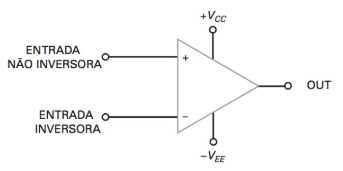
\includegraphics[height=.7\textheight, keepaspectratio]{../figs/cap02/ampop.PNG}
		\end{figure}		
	\end{frame}
	
	\begin{frame}{Modos de operação}
		\begin{itemize}
			\item Malha aberta
			\vspace{1em}
			\item Malha fechada
			\begin{itemize}
				\item Realimentação positiva
				\item Realimentação negativa
			\end{itemize}
		\end{itemize}
	\end{frame}
	
	\begin{frame}{Amplificador Operacional 741}
		\begin{figure}[hbtp]
		\centering
		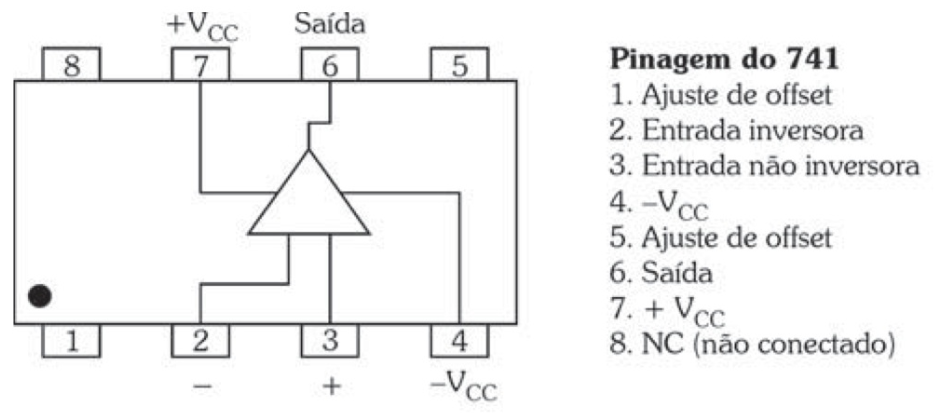
\includegraphics[height=.7\textheight, keepaspectratio]{../figs/cap02/ao741}
		\end{figure}		
	\end{frame}
	
	\section{Malha aberta}
	\begin{frame}{Definição}
		\begin{itemize}
			\item Ausência de realimentação (saída conectada a uma entrada) no circuito 
			\vspace{1em}
			\item Cálculo da tensão de saída
			\begin{equation*}
				V_S = A_{VOL}(V_{+}-V_{-})
			\end{equation*}
		\end{itemize}
	\end{frame}
	
	\begin{frame}{Saturação}
		\begin{itemize}
			\item Situação em que o ganho de tensão será limitado pela tensão de alimentação
		\end{itemize}
		
		\begin{figure}[hbtp]
		\centering
		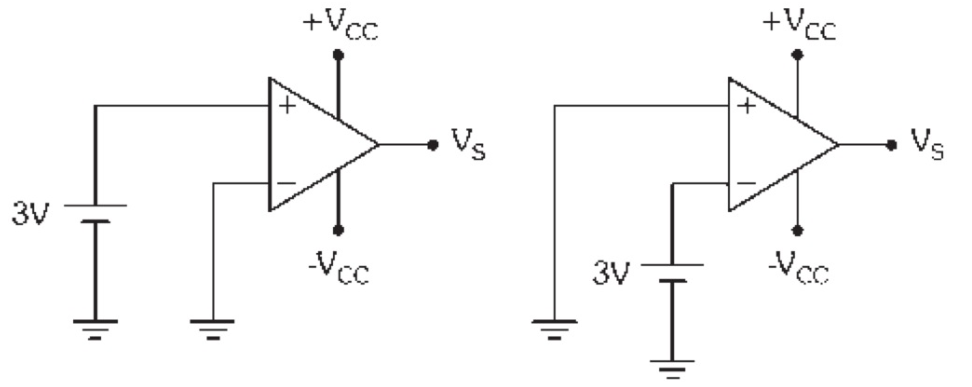
\includegraphics[height=.5\textheight, keepaspectratio]{../figs/cap02/saturacao}
		\end{figure}
	
	\end{frame}
	
	
	\section{Realimentação Positiva}
	
	\section{Realimentação Negativa}
	
	\subsection{Amplificador Inversor}
	
	\subsection{Amplificador Não Inversor}
	
	\subsection{Amplificador Somador}
	
	\subsection{Amplificador Subtrator}


	\begin{frame}{Bibliografia}
		\begin{itemize}
			\item MALVINO, A.; BATES, D.J. \textbf{Eletrônica – Volume II}, 8. ed., Porto Alegre, AMGH, 2016.
			\vspace{1em}
			\item ALBUQUERQUE, R.O.; SEABRA, A.C. \textbf{Utilizando Eletrônica com AO, SCR, TRIAC, UJT, PUT, CI 555, LDR, LED, IGBT e FET de Potência }  2. ed., São Paulo: Érica, 2012

		\end{itemize}
	\end{frame}	

	\begin{frame}{}
	\end{frame}

\end{document}
